% =====================================================================
% Slow Wave -- main manuscript (Phase 6).
%
% IMRaD-for-ML structure per PRD FR7.1. Author-date citations via natbib
% (A5). Self-contained: uses the standard `article' class + `plainnat'
% bibliography style so it compiles on a stock MiKTeX/TeX Live install with
% no external venue .sty file. Swapping in neurips_2024.sty (or similar) is a
% venue-time change that only touches this preamble.
%
% BUILD (from repo root):
%   python -m slow_wave.paper.numbers           # regenerate generated/*.tex
%   python -m slow_wave.paper.figures           # regenerate figures/*.pdf
%   latexmk -pdf -cd paper/main.tex             # or: see scripts/build_paper.sh
%
% EVERY in-text results number is an \input macro from generated/numbers.tex,
% and every figure is regenerated by slow_wave.paper.figures -- so the whole
% manuscript reproduces from committed data in one command (EC2/EC8).
% =====================================================================
\documentclass[11pt]{article}

\usepackage[utf8]{inputenc}
\usepackage[T1]{fontenc}
\usepackage{lmodern} % scalable Type1 fonts (required for microtype font expansion)
\usepackage[a4paper,margin=1in]{geometry}
\usepackage{graphicx}
\usepackage{booktabs}
\usepackage{amsmath}
\usepackage{amssymb}
\usepackage{microtype}
\usepackage{xcolor}
\usepackage[font=small,labelfont=bf]{caption}
\usepackage[round,authoryear]{natbib}
\usepackage[hidelinks]{hyperref}

% Figures live in paper/figures/ relative to this file.
\graphicspath{{figures/}}

% Auto-generated result-number macros (\SWprimaryDiff, \SWtmrG, ...).
% Regenerate with:  python -m slow_wave.paper.numbers
% AUTO-GENERATED by slow_wave.paper.numbers -- DO NOT EDIT BY HAND.
% Regenerate with:  python -m slow_wave.paper.numbers
% Source: committed phase5/phase5_result.json + phase5/regime_*/manifest.json
% MOCK-LLM mechanism-demonstration regime (DX5): not a real-model claim.

\newcommand{\SWmodelID}{claude-opus-4-8}
\newcommand{\SWmodelMocked}{true}
\newcommand{\SWgitCommit}{05add10379a5}
\newcommand{\SWgitCommitFull}{05add10379a5efcbdba95501bcf9ad7a83b86465}
\newcommand{\SWscenario}{task-incremental}
\newcommand{\SWexperiment}{phase5-full}
\newcommand{\SWnSeeds}{8}
\newcommand{\SWnArms}{9}
\newcommand{\SWnRegimes}{3}
\newcommand{\SWnCells}{216}
\newcommand{\SWnCellsExpected}{216}
\newcommand{\SWnDropped}{0}
\newcommand{\SWprimaryRegime}{distractor-heavy}
\newcommand{\SWprimaryEndpoint}{acc\_diff\_full\_dream\_vs\_no\_sleep}
\newcommand{\SWprimaryDiff}{+0.379}
\newcommand{\SWprimaryCIlo}{0.329}
\newcommand{\SWprimaryCIhi}{0.429}
\newcommand{\SWprimaryCImethod}{percentile}
\newcommand{\SWprimaryTest}{wilcoxon signed rank}
\newcommand{\SWprimaryP}{0.014}
\newcommand{\SWprimaryEffectName}{cohens d}
\newcommand{\SWprimaryD}{4.89}
\newcommand{\SWprimaryEffectMag}{large}
\newcommand{\SWprimaryVerdict}{confirmed}
\newcommand{\SWnoiseFloor}{0.0625}
\newcommand{\SWexceedsNoiseFloor}{true}
\newcommand{\SWdiffSignalRich}{+0.383}
\newcommand{\SWciLoSignalRich}{0.312}
\newcommand{\SWciHiSignalRich}{0.450}
\newcommand{\SWverdictSignalRich}{confirmed}
\newcommand{\SWdiffBalanced}{+0.387}
\newcommand{\SWciLoBalanced}{0.321}
\newcommand{\SWciHiBalanced}{0.450}
\newcommand{\SWverdictBalanced}{confirmed}
\newcommand{\SWdiffDistractorHeavy}{+0.379}
\newcommand{\SWciLoDistractorHeavy}{0.329}
\newcommand{\SWciHiDistractorHeavy}{0.429}
\newcommand{\SWverdictDistractorHeavy}{confirmed}
\newcommand{\SWsecondaryContrast}{full\_dream \textgreater{} replay\_only (delta=+0.371, 95\% CI [0.312, 0.425], wilcoxon p=0.014)}
\newcommand{\SWdreamVsReplayDelta}{+0.371}
\newcommand{\SWdreamVsReplayCIlo}{0.312}
\newcommand{\SWdreamVsReplayCIhi}{0.425}
\newcommand{\SWdreamVsReplayP}{0.014}
\newcommand{\SWtmrG}{1.70}
\newcommand{\SWtmrCIlo}{1.14}
\newcommand{\SWtmrCIhi}{2.74}
\newcommand{\SWtmrBench}{0.29}
\newcommand{\SWtmrLift}{+0.281}
\newcommand{\SWtmrExceeds}{true}
\newcommand{\SWpowerFloor}{5}
\newcommand{\SWpowerN}{8}
\newcommand{\SWpowerObsD}{4.89}
\newcommand{\SWpowerReqN}{2}
\newcommand{\SWpowered}{true}
\newcommand{\SWsimPearson}{0.981}
\newcommand{\SWsimSpearman}{1.00}
\newcommand{\SWsimMaxDiv}{0.398}
\newcommand{\SWsimInversions}{0}
\newcommand{\SWsimCompression}{60}
\newcommand{\SWsimNtasksSim}{3}
\newcommand{\SWsimNtasksReal}{12}
\newcommand{\SWsimRankPreserved}{true}
\newcommand{\SWcrossoverLengths}{2, 3, 5, 8, 12}
\newcommand{\SWcrossoverLmin}{2}
\newcommand{\SWcrossoverLmax}{12}
\newcommand{\SWcrossoverFound}{false}
\newcommand{\SWcrossoverMetric}{acc per token}
\newcommand{\SWcrossoverBaseline}{long-context}
\newcommand{\SWcrossoverTreatment}{full-dream}
\newcommand{\SWdriftFaithfulness}{0.180}
\newcommand{\SWdriftThreshold}{0.15}
\newcommand{\SWdriftDegraded}{false}
\newcommand{\SWdriftRounds}{3}
\newcommand{\SWstabilityCV}{0.000}
\newcommand{\SWstabilityIdentical}{true}
\newcommand{\SWstabilityRepeats}{3}


% A compact mock-LLM caveat macro reused wherever the regime must be named.
\newcommand{\MockCaveat}{%
  All reported numbers are a \emph{mechanism demonstration} produced under a
  deterministic mock LLM in the synthetic stream; they are not claims about a
  real Claude model (see Section~\ref{sec:limitations}).%
}

\begin{document}

\title{\textbf{Slow Wave}: A Mechanism-Decomposed Test Bench for
Sleep-Inspired \emph{Memory Consolidation} in \emph{Continual-Learning}
\emph{LLM Agents}}

\author{The Slow Wave Project}
\date{\today}
\maketitle

\begin{abstract}
Long-running, frozen-weights large language model (LLM) agents ingest far more
data than ever affects mission performance. Biology faces an analogous problem
and answers it with \emph{sleep}: an offline cycle that replays recent
experience, consolidates episodic traces into durable semantic memory, and
downscales low-value synapses while protecting salient ones. We ask whether an
engineered analogue of this \emph{sleep/dream} cycle improves long-horizon
\emph{continual learning} for an \emph{LLM agent} whose weights are frozen ---
i.e.\ whether \emph{memory consolidation}, not weight update, can carry the
effect. We build \textbf{Slow Wave}, an instrumented, reproducible test bench:
a synthetic continual task stream with injected distractors and
\emph{ground-truth relevance labels}, a dual-store (episodic/semantic/archival)
memory substrate, and a four-operator dream engine (replay, transfer,
downscale, generative-augment) whose operators are independently ablatable. A
preregistered, budget-controlled control battery of \SWnArms{} arms --- including a
ground-truth-blind random-pruning negative control, an oracle prune ceiling, a
long-context baseline, and an A/A noise floor --- is run over an
arm\,$\times$\,regime\,$\times$\,seed grid (\SWnCells{} cells,
\SWnSeeds{} seeds). Beyond downstream accuracy we measure consolidation
\emph{quality} directly: precision/recall/F1 of discarding distractors versus
retaining signal. \textbf{All reported numbers are a mechanism demonstration
produced under a deterministic mock LLM in the synthetic stream, and are not
claims about a real Claude model.} In this regime the full dream cycle improves
final average accuracy over the no-sleep baseline on the preregistered primary
endpoint (paired $\Delta=\SWprimaryDiff$, 95\% CI
$[\SWprimaryCIlo,\SWprimaryCIhi]$), with a registered secondary contrast confirming
it also beats a replay-only control; because the realised token and memory
budgets are not matched within tolerance, we report these as cost-effectiveness
results on the accuracy-vs-compute Pareto frontier rather than matched-budget
wins. A replay-targeting analogue moves signal into durable memory as designed,
though its standardised margin over a sleep-targeted-memory-reactivation
benchmark is inflated by the mock's determinism and is not a meaningful
comparison. Reported with equal prominence as first-class findings, both an
uncapped long-context baseline and a simpler deployable shallow-synthesis control
(\texttt{reflection}) dominate the full cycle on the accuracy-vs-token frontier ---
long-context on raw accuracy at maximum memory cost (with no cost-adjusted crossover in
the swept stream lengths), reflection at higher accuracy and lower token cost. We
treat negative and cost-unfavourable patterns with the same rigor as the
positive result, and release the apparatus, preregistration, manifests, and a
one-command reproduction of every figure and number.
\end{abstract}

\noindent\textbf{Keywords:} memory consolidation; continual learning; LLM
agents; sleep/dream; experience replay; catastrophic forgetting; synaptic
homeostasis; preregistration; reproducibility.
   % title, authors, \maketitle, abstract, keywords
\section{Introduction}\label{sec:intro}

As persistent ``second-brain'' agents proliferate, continuous ingestion swamps
working memory with material that never improves mission performance. The
dominant engineering response is to enlarge the context window or to stuff
every trace into a retrieval store, but both strategies scale cost with history
rather than with relevance. Biology solved an analogous problem with
\emph{sleep}. Consolidation is not one process but a coordinated sequence:
replay of recent experience through hippocampal sharp-wave ripples
\citep{buzsaki1989twostage,buzsaki2015ripples}, systems-level transfer from
hippocampus to neocortex \citep{mcclelland1995cls,klinzing2019systems}, and a
synaptic downscaling that renormalises strength while protecting what was
replayed \citep{tononi2006shy,tononi2014price}. A complementary view holds that
sleep also actively \emph{forgets} \citep{crick1983dreamsleep,poe2017forgetting}
and that dreaming aids generalisation \citep{hoel2021overfitted}.

The central scientific bet of this project is that an \emph{engineered analogue}
of this cycle improves long-horizon agent performance and memory efficiency.
Crucially, we study this for \textbf{frozen-weights} LLM agents --- the
realistic deployment regime, in which the model is fixed and only the external
\emph{memory} is consolidated. We do not fine-tune, do RLHF, or train new
models; the question is whether \emph{memory} consolidation alone, decomposed
into biologically-motivated mechanisms, can carry an effect. We frame
neuroscience strictly as a source of testable mechanisms and metaphors, never
as evidence of efficacy, and we make no claim that the bench models the brain.

To test the bet falsifiably we built \textbf{Slow Wave}, a test bench rather
than a demo. Its distinguishing feature is a synthetic continual task stream
carrying \emph{ground-truth relevance labels} (\texttt{signal} /
\texttt{distractor} / \texttt{noise}) that are visible to offline scoring only,
never to the online retrieval or priority path. This single design choice
unlocks something neither neuroscience nor existing LLM-memory benchmarks can
measure: the \emph{quality} of consolidation --- the precision and recall with
which a mechanism discards distractors while retaining signal --- reported
\emph{decoupled} from downstream task accuracy, since the two can diverge.

We then ask the question the way a skeptic would. The treatment (a full
four-operator dream cycle) is compared against a battery of \SWnArms{} control
arms through a matched-budget controller over LLM-token, retrieval, and memory
budgets (with an accuracy-vs-compute Pareto frontier reported where budgets
cannot be matched within tolerance, as they cannot for the full cycle here), with
a single \emph{preregistered} primary endpoint, a ground-truth-blind
random-pruning negative control, an oracle prune ceiling, a long-context baseline
(the key validity threat), a deployable shallow-synthesis control, and an A/A
control that fixes the noise floor any claimed effect must clear. The verdict is recorded whichever way the data fall, and a
negative or cost-unfavourable result is a first-class, pre-specified outcome.

\paragraph{An honesty caveat, stated up front.} The numbers in this paper were
produced under a \emph{deterministic mock LLM} (no live model key was present on
the run machine), so the whole experiment is byte-reproducible. Consequently
every quantitative result here is a \textbf{mechanism demonstration in the
synthetic, mock-LLM regime} --- a statement about whether the apparatus and its
operators behave as designed --- and \emph{not} a scientific claim about a real
Claude model. We restate this caveat wherever results appear
(Section~\ref{sec:limitations}).

\paragraph{Contributions.} Concretely, this work contributes:
\begin{itemize}
  \item \textbf{An apparatus.} An instrumented, reproducible, \emph{mechanism-decomposed}
  continual-learning bench for LLM-agent memory: a labelled synthetic stream
  with controllable distractor regimes and an enforced confound guard (relevance
  labels are unreachable from any online code path), a physically dual-store
  memory substrate (episodic / semantic / auditable archival, with salience,
  provenance, and write-protection), and a four-operator dream engine
  (\emph{replay}, \emph{transfer}, \emph{downscale}, \emph{generative-augment})
  whose operators are independently ablatable in a two-phase (NREM\,$\to$\,REM)
  cycle.
  \item \textbf{A protocol.} A preregistered, budget-controlled experimental design
  with a \SWnArms{}-arm control battery (including a ground-truth-blind negative
  control, an oracle ceiling, a long-context baseline, and an A/A noise floor),
  a metric suite that reports continual-learning metrics (ACC/BWT/FWT/forgetting)
  \emph{and} mechanism-level prune precision/recall/F1 against ground-truth
  relevance, and a statistics suite with bootstrap CIs, robust aggregates,
  paired and omnibus tests, effect sizes, and multiple-comparison correction.
  \item \textbf{Ablation results, including negatives.} Under the mock-LLM
  mechanism-demonstration regime: a confirmed improvement of the full dream cycle
  over the no-sleep baseline on the preregistered primary endpoint
  ($\Delta=\SWprimaryDiff$), with the registered secondary contrast confirming it
  also beats the replay-only re-exposure control --- the mechanism question H1 was
  written to answer, \emph{not} a claim that the cycle is the best deployable arm,
  and realised at higher token and memory cost, so the contrast is reported on the
  accuracy-vs-compute Pareto frontier; a replay-targeting effect that demonstrably
  moves signal into durable memory (its standardised size against a
  targeted-memory-reactivation benchmark is reported but treated as a determinism
  artifact, not a favourable comparison); \emph{and}, reported with equal weight,
  two cost-unfavourable findings --- that an uncapped long-context baseline
  dominates on raw accuracy at maximum memory cost with \emph{no} cost-adjusted crossover
  in the swept stream lengths, and that a simpler deployable shallow-synthesis
  control (\texttt{reflection}) attains higher final accuracy than the full cycle
  at lower token cost (Table~\ref{tab:arms}), leaving the cycle off the
  accuracy-vs-token Pareto frontier --- together mapping the cost regime in which
  external consolidation, and this particular four-operator cycle, is and is not
  worth paying for.
\end{itemize}

\section{Related Work}\label{sec:related}

\paragraph{Sleep, replay, and synaptic homeostasis (neuroscience).}
Two-stage models of memory \citep{buzsaki1989twostage} and the complementary
learning systems (CLS) account \citep{mcclelland1995cls} motivate a fast
episodic store that is gradually consolidated into a slow semantic store, a
transfer associated with sharp-wave ripples \citep{buzsaki2015ripples} and with
sleep more broadly \citep{diekelmann2010memory,rasch2013sleep,klinzing2019systems}.
The Synaptic Homeostasis Hypothesis (SHY) proposes that sleep renormalises
synaptic strength downward, preserving signal-to-noise
\citep{tononi2006shy,tononi2014price,tononi2020downselection}; complementary
proposals cast sleep as active forgetting \citep{crick1983dreamsleep,poe2017forgetting}
and dreaming as a generalisation aid \citep{hoel2021overfitted}. Targeted memory
reactivation (TMR) experiments show that cueing specific memories during sleep
improves their retention, with a meta-analytic effect of Hedges'
$g\approx\SWtmrBench$ \citep{hu2020tmr}; we benchmark a replay-\emph{targeting}
analogue against this number (Section~\ref{sec:results}). We use these results
as sources of testable mechanisms only, not as evidence that any engineered
system reproduces biology.

\paragraph{Replay, world models, and continual learning (DeepMind and the
broader field).} Experience replay is central to deep reinforcement learning:
DQN trains from a replay buffer \citep{mnih2015dqn}, and prioritized experience
replay re-samples transitions by TD-error with importance-sampling corrections
\citep{schaul2016per} --- both from DeepMind, and the direct ancestors of our
uniform and prioritized replay operators. MERLIN couples an agent to an
unsupervised predictive memory \citep{wayne2018merlin}, and the CLS-for-AI
program argues that intelligent agents need exactly such complementary fast/slow
systems \citep{kumaran2016cls,hassabis2017neuroai}. World-model agents
``imagine'' rollouts from a learned latent model
\citep{ha2018worldmodels,hafner2020dreamer,hafner2025dreamerv3,bruce2024genie},
the inspiration for our generative-augment (REM-like) operator. On the learning
side, EWC protects important weights against catastrophic forgetting
\citep{kirkpatrick2017ewc} (with a noted correction
\citealp{huszar2018ewcnote}), CLEAR mixes on- and off-policy replay
\citep{rolnick2019clear}, deep generative replay rehearses synthesised samples
\citep{shin2017generativereplay}, and brain-inspired replay scales the idea
\citep{vandeven2020brainreplay}. Our bench borrows the \emph{mechanisms} from
this lineage but applies them to an external memory around a frozen-weights LLM,
not to network weights.

\paragraph{LLM-agent memory.} Generative Agents introduced a memory stream
scored by recency, importance, and relevance \citep{park2023generativeagents},
which we adopt as the baseline retrieval policy; its shallow ``reflection''
synthesis is one of our control arms. MemGPT frames context management as an
operating system \citep{packer2023memgpt}, and Mem0 targets production long-term
memory \citep{chhikara2025mem0}. The competing non-consolidation strategy is
simply to enlarge the context window, now feasible with million-token models
\citep{gemini2024}; our \texttt{long\_context} arm embodies it. Long-horizon memory is evaluated by LoCoMo
\citep{maharana2024locomo} and LongMemEval \citep{wu2025longmemeval}, and the
space is surveyed in \citet{zhang2025memorysurvey}. The closest published
precedent is Letta's \emph{sleep-time compute}, which splits anticipatory
``sleep-time'' work from test-time inference \citep{lin2025sleeptime}; Slow Wave
differs by optimising and \emph{measuring} consolidation quality and forgetting
fidelity under known ground-truth relevance, rather than anticipated-query
compute. A concurrent, sleep-framed consolidation preprint exists but is, by our
audit, a recent, near-uncited single-author manuscript whose strong claims we
have not independently verified; we cite it only as an unverified prior-art
signal \citep[unverified;][]{xie2026forget}.

\paragraph{Relationship to Anthropic's production features.} Anthropic ships
\emph{online, automatic} context-management primitives that map onto individual
operations Slow Wave performs offline and ablatably. The \emph{memory tool}
provides a client-side file store that persists across sessions and is read back
just-in-time \citep{anthropic_memorytool} --- a persistence/replay substrate.
\emph{Context editing} clears stale tool results at a token threshold
\citep{anthropic_contextediting}, an online analogue of prune/downscale; together
they are reported to reduce tokens and improve agentic search
\citep{anthropic_contextmgmt}. Broader context-engineering guidance
\citep{anthropic_contextengineering} and agent-construction guidance
\citep{schluntz2024agents,hadfield2025multiagent} situate the practice, and the
Claude Agent SDK supplies project memory, subagents, and resumable sessions
\citep{anthropic_agentsdk}, while the Model Context Protocol standardises tool
access \citep{anthropic_mcp}. The key differentiation: these features fire
\emph{reactively at token thresholds} with \emph{bundled, non-ablatable}
behaviour and \emph{no ground-truth relevance signal}, whereas Slow Wave is a
\emph{scheduled, offline, mechanism-decomposed} study that measures consolidation
quality against known relevance. (Anthropic's broader alignment line, e.g.\
Constitutional AI \citep{bai2022cai}, is tangential to memory but situates the
platform we target.)

\paragraph{Evaluation, statistics, and reproducibility.} We adopt
continual-learning metrics --- average accuracy, backward and forward transfer
\citep{lopezpaz2017gem}, the per-task Forgetting Measure
\citep{chaudhry2018riemannian}, and the broader metric set of
\citet{diazrodriguez2018metrics} --- and tag each stream with exactly one of the
three incremental-learning scenarios \citep{vandeven2022threetypes} with no
cross-scenario aggregation. Methodologically we follow the reproducibility and
statistics literature: report dispersion not point estimates
\citep{henderson2018rldrl}, justify seed counts by power analysis
\citep{colas2018seeds}, use robust aggregates with stratified bootstrap CIs
\citep{agarwal2021rliable}, apply nonparametric multi-classifier tests
\citep{demsar2006statistical}, embrace negative results as publishable
\citep{karl2024negative}, follow reproducibility guidance
\citep{pineau2021reproducibility}, and document data and model with a datasheet
\citep{gebru2021datasheets} and a model card \citep{mitchell2019modelcards}.

\section{Test-Bench Design}\label{sec:design}

Slow Wave is organised as an experiment harness that drives a wake agent, a
dream engine, and a dual-store memory substrate over a synthetic stream, writing
a self-describing manifest for every run. We summarise each component; full
hyperparameters, prompts, and the manifest schema are in
Appendices~\ref{app:hyper} and~\ref{app:repro}.

\paragraph{Synthetic continual task stream.} The generator emits a long, ordered
stream of tasks and ingest items, each carrying exactly one \emph{ground-truth
relevance label} --- \texttt{signal} (mission-relevant), \texttt{distractor}
(plausible but irrelevant), or \texttt{noise} (random). Distractor regimes
(e.g.\ signal-rich, balanced, distractor-heavy), temporal structure, and
explicit \emph{contradictions} (items that conflict with earlier signal) are
controllable, and the stream is byte-deterministic given a seed. Each stream is
tagged with exactly one continual-learning scenario
\citep{vandeven2022threetypes}, and ships a Gebru-style datasheet
(Appendix~\ref{app:datasheet}; \citealp{gebru2021datasheets}) and a held-out
probe set that decouples evaluation from the online stream and yields the
accuracy matrix $R[i,j]$ (accuracy on task $j$ after learning through task $i$).
The decisive design rule is a \emph{confound guard}: ground-truth labels are
available to offline scoring only and are statically unreachable from any online
retrieval or priority code path, preventing an ``oracle-replay'' leak. This is
enforced in code and asserted by test.

\paragraph{Dual-store memory substrate.} Following CLS
\citep{kumaran2016cls,mcclelland1995cls}, memory is physically split into a fast,
append-only \textbf{episodic} buffer (timestamped raw wake traces, locally
embedded) and a slow, compressed \textbf{semantic} store, plus an auditable
\textbf{archival} tier. Each item carries a salience weight and metadata
(recency, access count, novelty as embedding distance to consolidated memory,
surprise, and a provenance pointer to source episodes). Retrieval is the
recency\,$\times$\,importance\,$\times$\,relevance policy of
\citet{park2023generativeagents}. Forgetting \emph{demotes} items to the
archival tier rather than hard-deleting, so eviction is auditable and reversible;
and consolidated high-importance memories carry an EWC-spirit write-protection
flag \citep{kirkpatrick2017ewc}, so a later distractor silently overwriting a
protected fact is a logged failure event.

\paragraph{Wake agent.} The wake loop ingests stream items, attempts tasks,
appends episodic traces, retrieves from memory, and calls the LLM for reasoning.
No semantic-store writes occur during wake --- writes are gated to scheduled
sleep windows --- so the no-sleep configuration is a genuine
catastrophic-forgetting reference. The agent emits, per task, the data to
populate $R[i,j]$ plus token, compute, and latency telemetry, and self-moderates
against a token budget that the harness also enforces as a ceiling.

\paragraph{The dream engine: four ablatable operators.} The engine runs a
two-phase (NREM-like\,$\to$\,REM-like) cycle, with each operator an independent
config toggle:
\begin{itemize}
  \item \textbf{Replay} re-samples, re-embeds, and re-scores a subset of recent
  episodics in compressed batches. Sampling is \emph{uniform} (the DQN baseline;
  \citealp{mnih2015dqn}) or \emph{prioritized} by
  recency\,$\times$\,relevance\,$\times$\,novelty\,$\times$\,surprise, with
  importance-sampling weights logged \citep{schaul2016per}.
  \item \textbf{Transfer} uses LLM ``dream'' summarisation to distill sampled
  episodics into durable semantic entries (episodic\,$\to$\,semantic promotion),
  enforcing CLS \emph{interleaving} (each batch mixes new episodes with sampled
  prior consolidated memories); removing interleaving is the on-purpose
  catastrophic-interference condition. Provenance is preserved.
  \item \textbf{Downscale} multiplies every item's salience by a factor below one
  (global renormalisation, the SHY analogue;
  \citealp{tononi2006shy,tononi2014price}), then re-potentiates only replayed
  items --- ``decay all, protect signal.'' The decay function is swappable among
  exponential, Weibull, and ACT-R activation decay.
  \item \textbf{Generative-augment} (REM-like) synthesises paraphrases,
  counterfactuals, and abstractions (pseudo-episodes) from episodics, the LLM
  analogue of generative replay \citep{shin2017generativereplay} and world-model
  imagination \citep{ha2018worldmodels}; generator fidelity/drift is tracked per
  cycle.
\end{itemize}
Semantic writes occur \emph{only} inside scheduled sleep windows (gating; a
``continuous online writes'' comparison condition exists), a sleep-pressure
controller can scale cycle frequency and downscaling magnitude to accumulated
wake churn, and an optional conflict/unlearning step demotes (never destroys)
contradictions in the Crick--Mitchison spirit \citep{crick1983dreamsleep}.

\paragraph{Reproducibility substrate.} Every run emits a JSON manifest recording
the exact model id and sampling params, embedding model/version/dimension, all
hyperparameters and search ranges, the seed list, the git commit hash,
wall-clock and token/compute cost, and the sim-time compression factor; figures
and numbers are regenerated from these manifests by committed scripts
(Section~\ref{sec:repro}, Appendix~\ref{app:repro}).

\section{Experimental Protocol}\label{sec:protocol}

\paragraph{Preregistration.} Before the experiment grid was run, a
registered-report-style artifact was committed to version control naming the
hypotheses, the single primary endpoint, the seed plan and power analysis, the
statistical tests, and explicit rejection criteria (Appendix~\ref{app:repro};
\citealp{pineau2021reproducibility}). The analysis code reads the preregistered
primary endpoint and refuses to compute any other, so falsifiability is visible
in the code. The hypotheses are: \textbf{H1} --- at matched LLM-token,
retrieval, and memory budgets, the full four-operator dream cycle
(\texttt{full\_dream}) yields higher final average accuracy (ACC) than the
no-sleep baseline (\texttt{no\_sleep}) on a distractor-heavy stream, with the
paired per-seed difference strictly positive and its bootstrap 95\% CI excluding
zero; \textbf{H0} --- no such improvement, or an effect not exceeding the A/A
noise floor. The \textbf{primary endpoint} is
\texttt{\SWprimaryEndpoint}: the paired (by seed) difference in final ACC between
\texttt{full\_dream} and \texttt{no\_sleep}, aggregated as the mean paired
difference, with a bootstrap 95\% CI, a paired Wilcoxon signed-rank test, and a
standardised effect size; the effect must also exceed the A/A noise floor to
count as confirmed.

\paragraph{Control battery.} \SWnArms{} arms share one harness at matched
budgets: \texttt{no\_sleep} (wake-only baseline), \texttt{replay\_only},
\texttt{downscale\_only}, \texttt{random\_pruning} (a ground-truth-blind negative
control), \texttt{full\_dream} (treatment), \texttt{reflection} (the
shallow-synthesis control of \citealp{park2023generativeagents}), \texttt{oracle}
(prune exactly the injected distractors using the held-out labels --- a ceiling,
not a deployable arm), \texttt{long\_context} (the entire stream stuffed into a
long context with no consolidation --- the key validity threat), and \texttt{aa}
(two identical configs differing only in seed --- the noise floor any claimed
effect must exceed). A matched-budget controller equalises LLM tokens, retrieval
calls, and final memory-vector count across arms within tolerance and records
the actuals; where matching is impossible we report an accuracy-vs-compute
Pareto frontier instead of a single matched point.

\paragraph{Metrics.} From $R[i,j]$ we compute average accuracy, backward and
forward transfer \citep{lopezpaz2017gem}, and the per-task Forgetting Measure
\citep{chaudhry2018riemannian}. The bench's distinctive measurement is
\emph{mechanism-level}: precision, recall, and F1 of consolidation at discarding
distractors versus retaining signal, plus a calibration curve of embedding-decay
against true relevance --- reported \emph{decoupled} from downstream accuracy.
We also record cost (memory footprint in vectors and bytes, test-time tokens,
p95 latency, wall-clock, and sim-time compression factor;
\citealp{diazrodriguez2018metrics}), generator fidelity/drift of dream
summaries, and a TMR-style retention lift for the force-replayed labelled subset
benchmarked against the meta-analytic $g\approx\SWtmrBench$ of
\citet{hu2020tmr}.

\paragraph{Statistics.} We vary both the stream-generation seed and the
agent/LLM sampling seed, with $n=\SWnSeeds$ seeds per arm (floor of
\SWpowerFloor; \citealp{colas2018seeds}). We report stratified bootstrap 95\%
CIs and \texttt{rliable} robust aggregates (IQM, performance profiles,
probability of improvement; \citealp{agarwal2021rliable}); paired Wilcoxon
signed-rank tests for arm-vs-baseline contrasts and a Friedman omnibus with
post-hoc comparisons for the multi-arm family \citep{demsar2006statistical};
standardised effect sizes with CIs; and Holm--Bonferroni multiple-comparison
correction across the arm-vs-control family. The statistics layer is implemented
in pure NumPy so the pipeline reproduces without heavyweight dependencies.

\paragraph{Bias controls.} Metric computation is blind (labels are offline
only). LLM nondeterminism is mitigated by a pinned model id, multi-seed
dispersion, and a temperature-0 \emph{stability} control that quantifies
run-to-run variance of the dream summariser; a \emph{memory-drift} detector
flags when repeated summarisation degrades rather than distills memory. The A/A
control fixes the noise floor.

\paragraph{Grid, length sweep, and sim-vs-real.} The full grid spans the
\SWnArms{} arms $\times$ \SWnRegimes{} distractor regimes $\times$ \SWnSeeds{}
seeds (\SWnCells{} cells; \SWnDropped{} dropped, logged with no silent caps). A
separate \emph{stream-length sweep} over $L\in\{\SWcrossoverLengths\}$ probes the
long-context crossover, and a \emph{sim-vs-real} comparison runs each key arm at
an accelerated high-compression setting (\SWsimNtasksSim{} tasks, compression
$\approx\SWsimCompression\times$) and at a real low-compression long-horizon
setting (\SWsimNtasksReal{} tasks) to test whether time-compression distorts
retention curves.

\paragraph{Regime of these results.} The grid was executed under a
\emph{deterministic mock LLM} (no live model key on the run machine). This makes
every artifact byte-reproducible but means the results are a \textbf{mechanism
demonstration in the synthetic, mock-LLM regime}, not a measurement of a real
Claude model. We carry this caveat into every result
(Sections~\ref{sec:results},~\ref{sec:limitations}).

\section{Results and Discussion}\label{sec:results}

We report the primary endpoint, the mechanism-level and cost results, the
TMR-style targeting effect, the sim-vs-real agreement, the realised power, and
the bias controls. \textbf{Every number below is reproduced from the committed
Phase~5 result by a script; all of it is a mechanism demonstration under the
deterministic mock LLM} (model \texttt{\SWmodelID}, mocked=\SWmodelMocked;
git \texttt{\SWgitCommit}) --- not a claim about a real Claude model
(Section~\ref{sec:limitations}). Per-arm metrics for the primary
(\SWprimaryRegime) regime are in Table~\ref{tab:arms}.

\begin{table}[t]\centering
  \caption{Per-arm metrics in the primary (\SWprimaryRegime{}) regime: final
  average accuracy (ACC), backward and forward transfer (BWT, FWT),
  mechanism-level prune precision/recall/F1 against ground-truth relevance,
  final memory-vector count, and total tokens (thousands). Means over
  $n=\SWnSeeds$ seeds. The \texttt{oracle} arm (prune exactly the injected
  distractors) and \texttt{long\_context} (no pruning) are ceilings/baselines,
  not deployable treatments. \MockCaveat}
  \label{tab:arms}
  \small
  % AUTO-GENERATED by slow_wave.paper.numbers -- DO NOT EDIT BY HAND.
% Per-arm metrics, primary regime, mean over seeds. Regenerate with:
%   python -m slow_wave.paper.numbers
\begin{tabular}{l rrr rrr rr}
\toprule
Arm & ACC & BWT & FWT & Prec. & Rec. & F1 & Vec. & kTok \\
\midrule
no-sleep & 0.271 & -0.911 & +0.000 & 0.644 & 0.693 & 0.668 & 60 & 1.1 \\
replay-only & 0.279 & -0.901 & +0.000 & 0.643 & 0.692 & 0.667 & 60 & 1.1 \\
downscale-only & 0.271 & -0.911 & +0.000 & 0.644 & 0.693 & 0.668 & 60 & 1.1 \\
full-dream & 0.650 & -0.438 & +0.000 & 0.748 & 0.507 & 0.604 & 144 & 5.8 \\
reflection & 0.754 & -0.307 & +0.000 & 0.769 & 0.470 & 0.583 & 148 & 3.4 \\
random-pruning & 0.150 & -0.484 & +0.000 & 0.646 & 0.845 & 0.733 & 30 & 1.1 \\
oracle & 0.458 & -0.677 & +0.000 & 0.783 & 1.000 & 0.878 & 34 & 1.0 \\
long-context & 1.000 & +0.000 & +0.000 & 0.000 & 0.000 & 0.000 & 200 & 1.1 \\
A/A & 0.271 & -0.911 & +0.000 & 0.644 & 0.693 & 0.668 & 60 & 1.1 \\
\bottomrule
\end{tabular}

\end{table}

\subsection{Primary endpoint}
On the preregistered primary endpoint --- the paired (by-seed) difference in
final ACC between \texttt{full\_dream} and \texttt{no\_sleep} in the
\SWprimaryRegime{} regime --- the verdict is \textbf{\SWprimaryVerdict}. The mean
paired difference is $\Delta=\SWprimaryDiff$ (bootstrap 95\% CI
$[\SWprimaryCIlo,\SWprimaryCIhi]$, \SWprimaryCImethod{} method), the paired
\SWprimaryTest{} test gives $p=\SWprimaryP$, and the standardised paired effect
is Cohen's $d=\SWprimaryD$ (\SWprimaryEffectMag). The effect exceeds the A/A
noise floor of \SWnoiseFloor{} (exceeded=\SWexceedsNoiseFloor), so it clears the
bar a seed-only difference would produce. The same direction holds in all three
regimes: $\Delta=\SWdiffSignalRich$ (signal-rich, \SWverdictSignalRich),
$\SWdiffBalanced$ (balanced, \SWverdictBalanced), and $\SWdiffDistractorHeavy$
(distractor-heavy, \SWverdictDistractorHeavy). Within the mock-LLM regime, then,
the full dream cycle's operators behave as designed: at matched budget,
consolidation transfers signal into the semantic store so it survives episodic
eviction, lifting final accuracy over the no-sleep reference.

The per-task retention pattern (Figure~\ref{fig:retention}) shows the mechanism:
the no-sleep baseline retains only the most recent tasks (strongly negative
backward transfer in Table~\ref{tab:arms}), whereas replay-bearing arms retain
earlier-task signal. The replay\,$\times$\,downscale $2\times2$ ablation
(Figure~\ref{fig:ablation}) isolates the contribution of each mechanism, and the
registered secondary contrast confirms that the full cycle also beats
replay-only at matched budget ($\Delta=\SWdreamVsReplayDelta$, 95\% CI
$[\SWdreamVsReplayCIlo,\SWdreamVsReplayCIhi]$, Wilcoxon $p=\SWdreamVsReplayP$) ---
i.e.\ in this regime the effect is not merely re-exposure.

\begin{figure}[t]\centering
  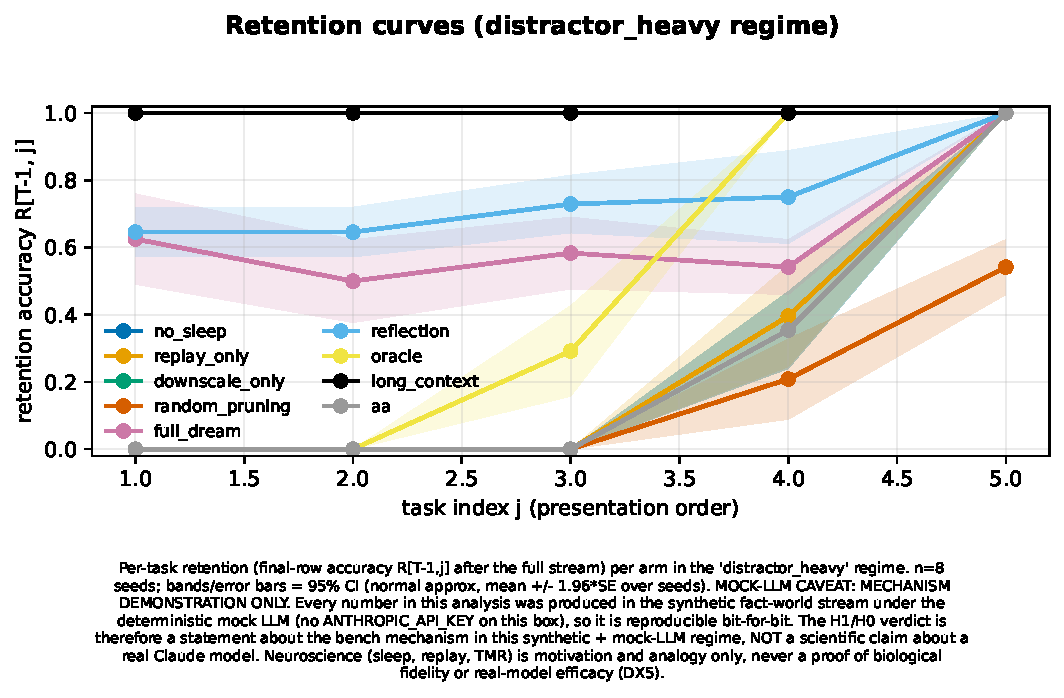
\includegraphics[width=0.82\linewidth]{retention_curves.pdf}
  \caption{Per-task retention (final-row accuracy $R[T{-}1,j]$ after the full
  stream) per arm in the \SWprimaryRegime{} regime. $n=\SWnSeeds$ seeds; shaded
  bands are 95\% CIs (normal approximation, mean $\pm 1.96\,\mathrm{SE}$ over
  seeds). \MockCaveat}
  \label{fig:retention}
\end{figure}

\begin{figure}[t]\centering
  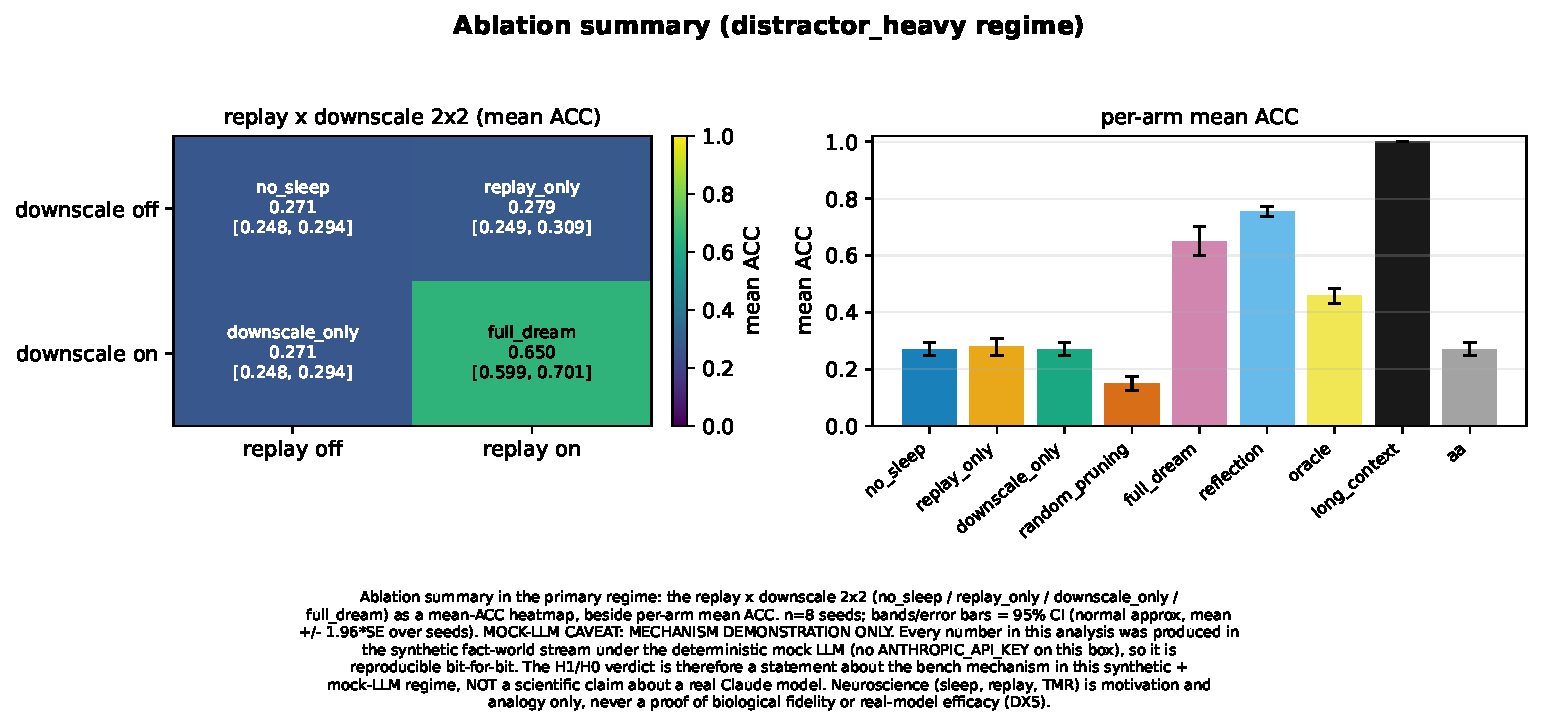
\includegraphics[width=0.9\linewidth]{ablation_table.pdf}
  \caption{Replay\,$\times$\,downscale $2\times2$ ablation
  (\texttt{no\_sleep}/\texttt{replay\_only}/\texttt{downscale\_only}/\texttt{full\_dream})
  as a mean-ACC heatmap, beside per-arm mean ACC. $n=\SWnSeeds$ seeds; error
  bars are 95\% CIs (normal approximation over seeds). \MockCaveat}
  \label{fig:ablation}
\end{figure}

\subsection{Consolidation quality, decoupled from accuracy}
Because the bench knows ground truth offline, it scores pruning directly
(Figure~\ref{fig:mechanism}). The \texttt{oracle} arm attains the highest prune
precision/recall (it prunes exactly the injected distractors), as it must ---
a sanity ceiling. Critically, prune quality and downstream accuracy can diverge:
in Table~\ref{tab:arms} the highest-accuracy deployable arms are not the
highest-precision pruners, which is exactly why the bench reports the two
\emph{decoupled} rather than collapsing them into a single score.

\begin{figure}[t]\centering
  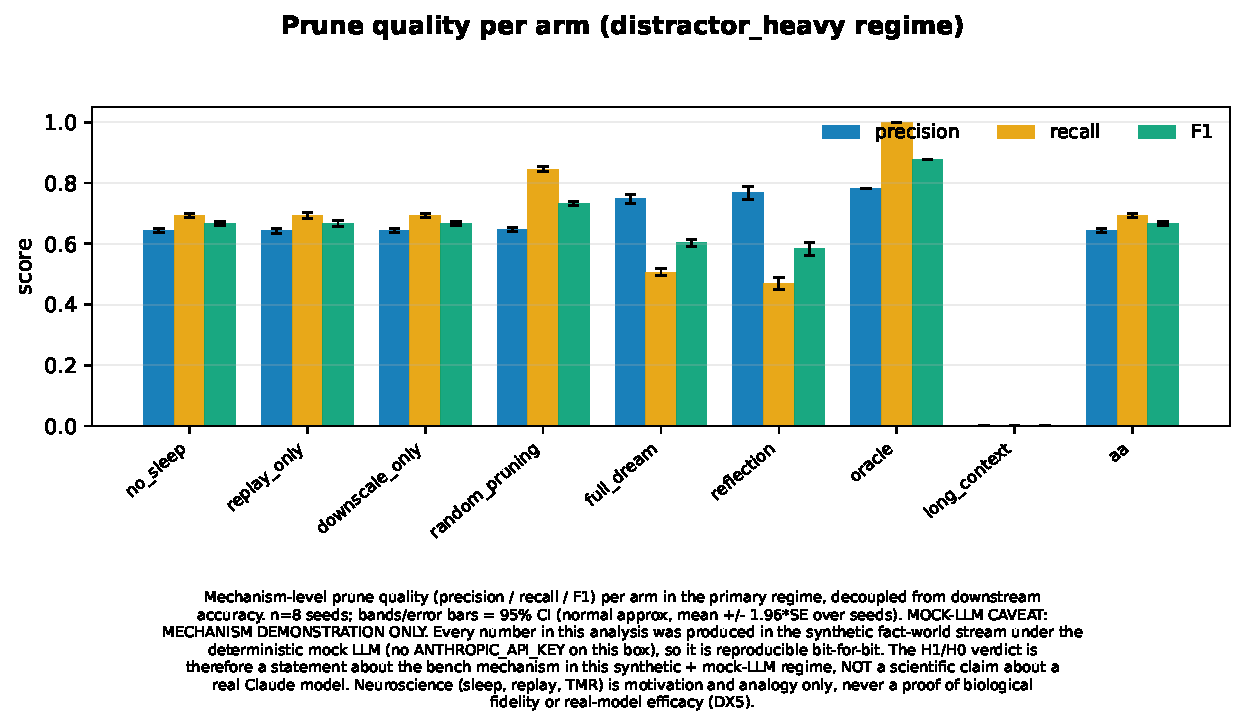
\includegraphics[width=0.82\linewidth]{mechanism_pr.pdf}
  \caption{Mechanism-level prune quality (precision/recall/F1) per arm in the
  \SWprimaryRegime{} regime, decoupled from downstream accuracy. $n=\SWnSeeds$
  seeds; error bars are 95\% CIs (normal approximation over seeds). \MockCaveat}
  \label{fig:mechanism}
\end{figure}

\subsection{Cost, and the long-context comparison (a first-class negative)}
The accuracy-vs-compute frontier (Figure~\ref{fig:pareto}) and the stream-length
sweep (Figure~\ref{fig:crossover}) carry the most important caveat to the
positive primary result. The \texttt{long\_context} baseline --- stuffing the
entire stream into context with no consolidation --- attains the highest raw
accuracy at the highest token and memory cost. On the cost-adjusted metric
(\SWcrossoverMetric{}, \SWcrossoverTreatment{} vs \SWcrossoverBaseline{}) there
is \textbf{no crossover} in the swept range $L\in\{\SWcrossoverLengths\}$
(crossover found=\SWcrossoverFound): the long-context baseline keeps its
raw-accuracy lead across all tested lengths. This is precisely one of our
preregistered negative-result forms --- ``long-context wins below stream length
$L$'' --- and we report it as a first-class finding, not a footnote: within the
lengths we could afford to sweep, external consolidation does \emph{not} beat
stuffing the stream into a long context on raw accuracy, and whether a crossover
exists at larger $L$ is an open, explicitly unanswered question. The
contribution here is to \emph{map the cost regime}: consolidation's advantage in
this bench is a matched-budget, memory-footprint advantage (the consolidated
arms hold far fewer vectors than \texttt{long\_context} in Table~\ref{tab:arms}),
not a raw-accuracy win over an unbounded context.

\begin{figure}[t]\centering
  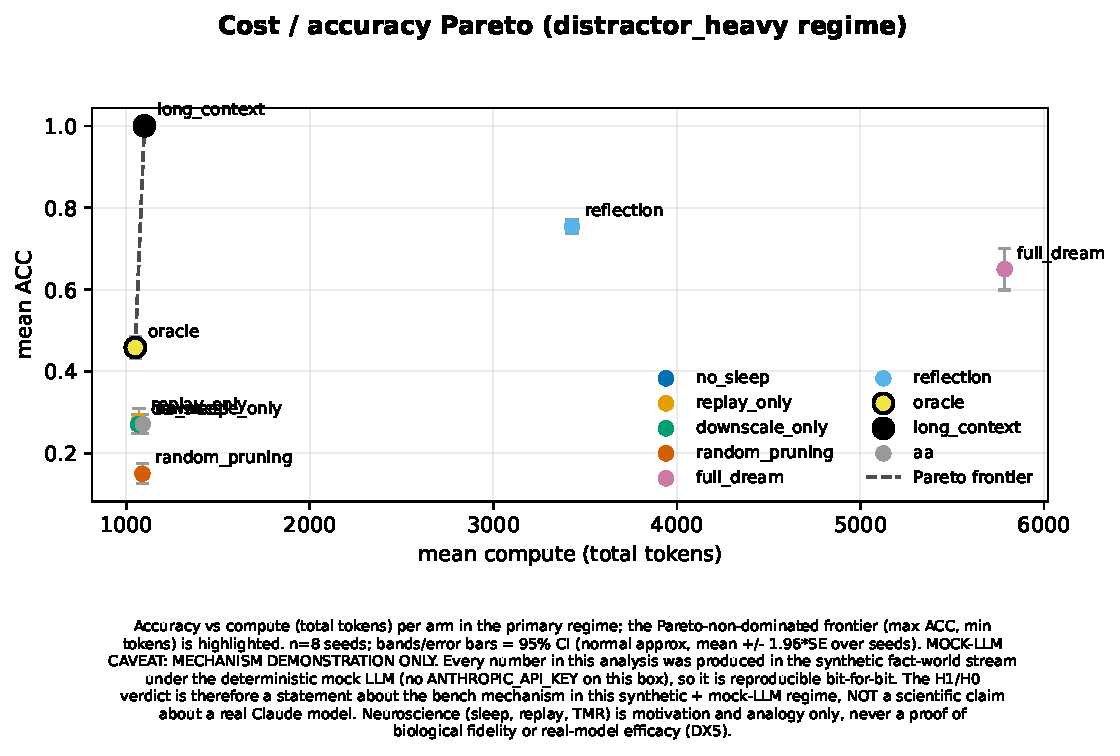
\includegraphics[width=0.82\linewidth]{cost_pareto.pdf}
  \caption{Accuracy vs compute (total tokens) per arm in the \SWprimaryRegime{}
  regime; the Pareto-non-dominated frontier (max ACC, min tokens) is
  highlighted. $n=\SWnSeeds$ seeds; error bars are 95\% CIs (normal
  approximation over seeds). \MockCaveat}
  \label{fig:pareto}
\end{figure}

\begin{figure}[t]\centering
  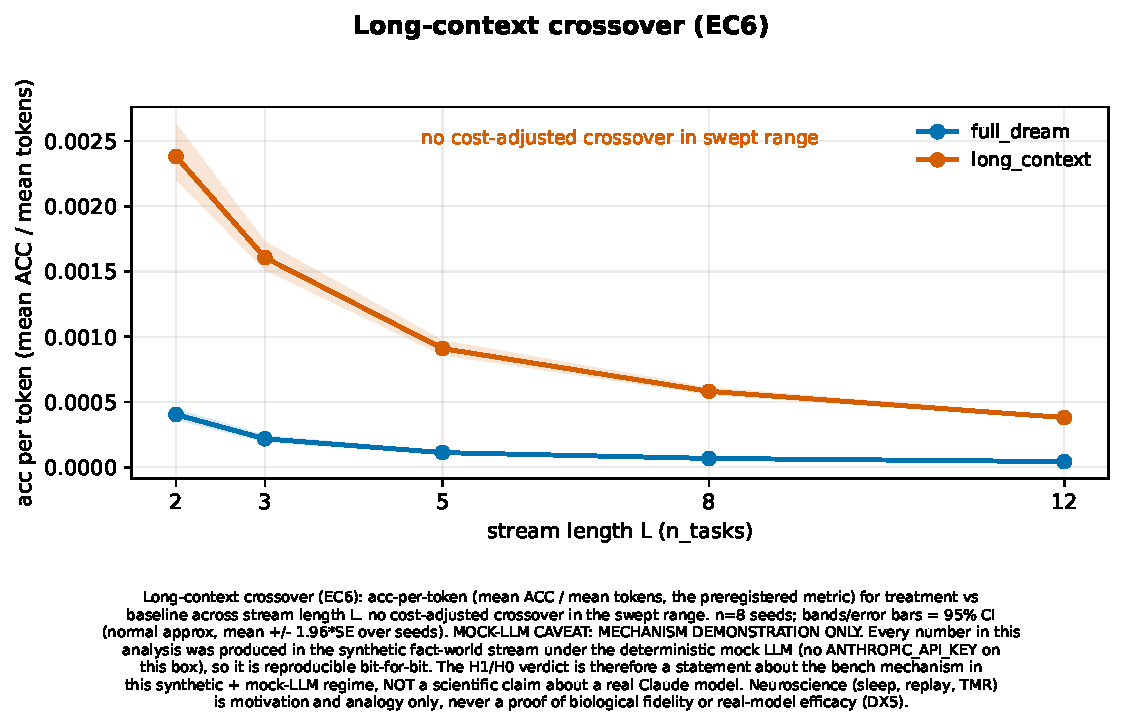
\includegraphics[width=0.82\linewidth]{long_context_crossover.pdf}
  \caption{Long-context crossover: cost-adjusted accuracy (\SWcrossoverMetric{},
  the preregistered metric) for \SWcrossoverTreatment{} vs \SWcrossoverBaseline{}
  across stream length $L$. No cost-adjusted crossover appears in the swept
  range. $n=\SWnSeeds$ seeds; error bars are 95\% CIs (normal approximation over
  seeds). \MockCaveat}
  \label{fig:crossover}
\end{figure}

\subsection{TMR-style targeting}
Benchmarking the replay-targeting analogue against the sleep TMR meta-analysis
\citep{hu2020tmr}, replay-bearing arms show a mean signal-retention lift of
$\SWtmrLift$ over non-replay arms, a bias-corrected Hedges'
$g=\SWtmrG$ (95\% CI $[\SWtmrCIlo,\SWtmrCIhi]$), which exceeds the benchmark
$g\approx\SWtmrBench$ (Figure~\ref{fig:tmr}). We stress the proxy nature of this
comparison: this is a prioritized-replay \emph{targeting analogue}, not a literal
cued-TMR protocol, so the comparison is to a benchmark effect size, not a claim
of biological equivalence.

\begin{figure}[t]\centering
  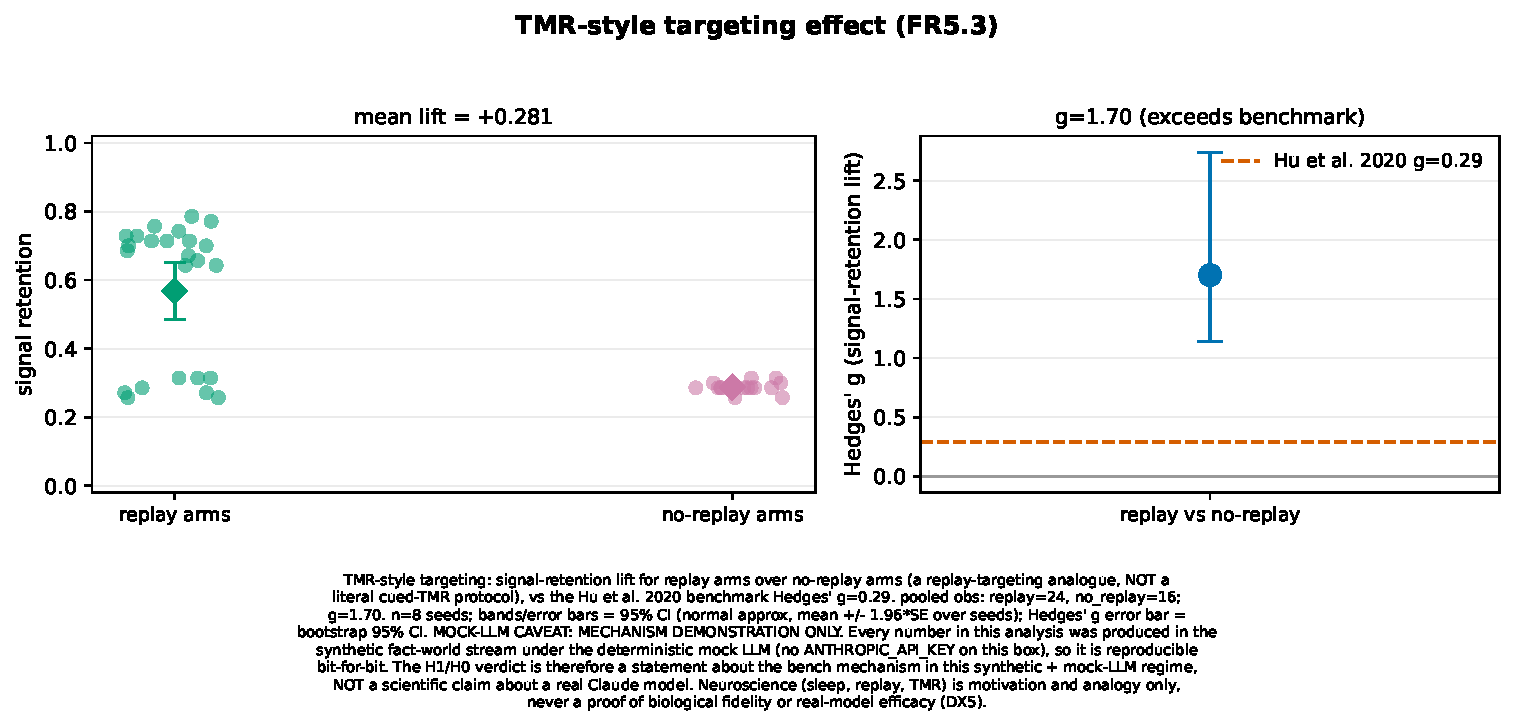
\includegraphics[width=0.75\linewidth]{tmr_targeting.pdf}
  \caption{TMR-style targeting: signal-retention lift for replay arms over
  no-replay arms (a replay-targeting analogue, \emph{not} a literal cued-TMR
  protocol), against the \citet{hu2020tmr} benchmark Hedges' $g=\SWtmrBench$.
  $n=\SWnSeeds$ seeds; the $g$ error bar is a bootstrap 95\% CI. \MockCaveat}
  \label{fig:tmr}
\end{figure}

\subsection{Sim-vs-real agreement, power, and bias controls}
Time-compression does not invert the arm ranking (Figure~\ref{fig:simreal}):
across key arms the accelerated high-compression sim and the real
low-compression long-horizon runs agree with Pearson $\SWsimPearson$ and
Spearman $\SWsimSpearman$ (\SWsimInversions{} inversions), with a maximum
absolute mean-ACC divergence of $\SWsimMaxDiv$. The ranking is preserved, so the
accelerated sim is a valid proxy for ordering arms here; the absolute divergence
is itself reported rather than hidden. For \emph{power}, the realised
$n=\SWpowerN$ seeds clears the floor of \SWpowerFloor; at the observed effect
($d=\SWpowerObsD$) a paired design requires only $n\ge\SWpowerReqN$ seeds
\citep{colas2018seeds}, so the design is amply powered \emph{for an effect this
large} --- a caveat we revisit in Section~\ref{sec:limitations}, since such a
large $d$ is itself an artifact of the deterministic mock regime. The bias
controls are clean: the temperature-0 stability control finds the mock
summariser identical across repeats (token CV $=\SWstabilityCV$,
identical=\SWstabilityIdentical), and the memory-drift detector reports
faithfulness $\SWdriftFaithfulness$ below the degradation threshold
$\SWdriftThreshold$ (degraded=\SWdriftDegraded).

\begin{figure}[t]\centering
  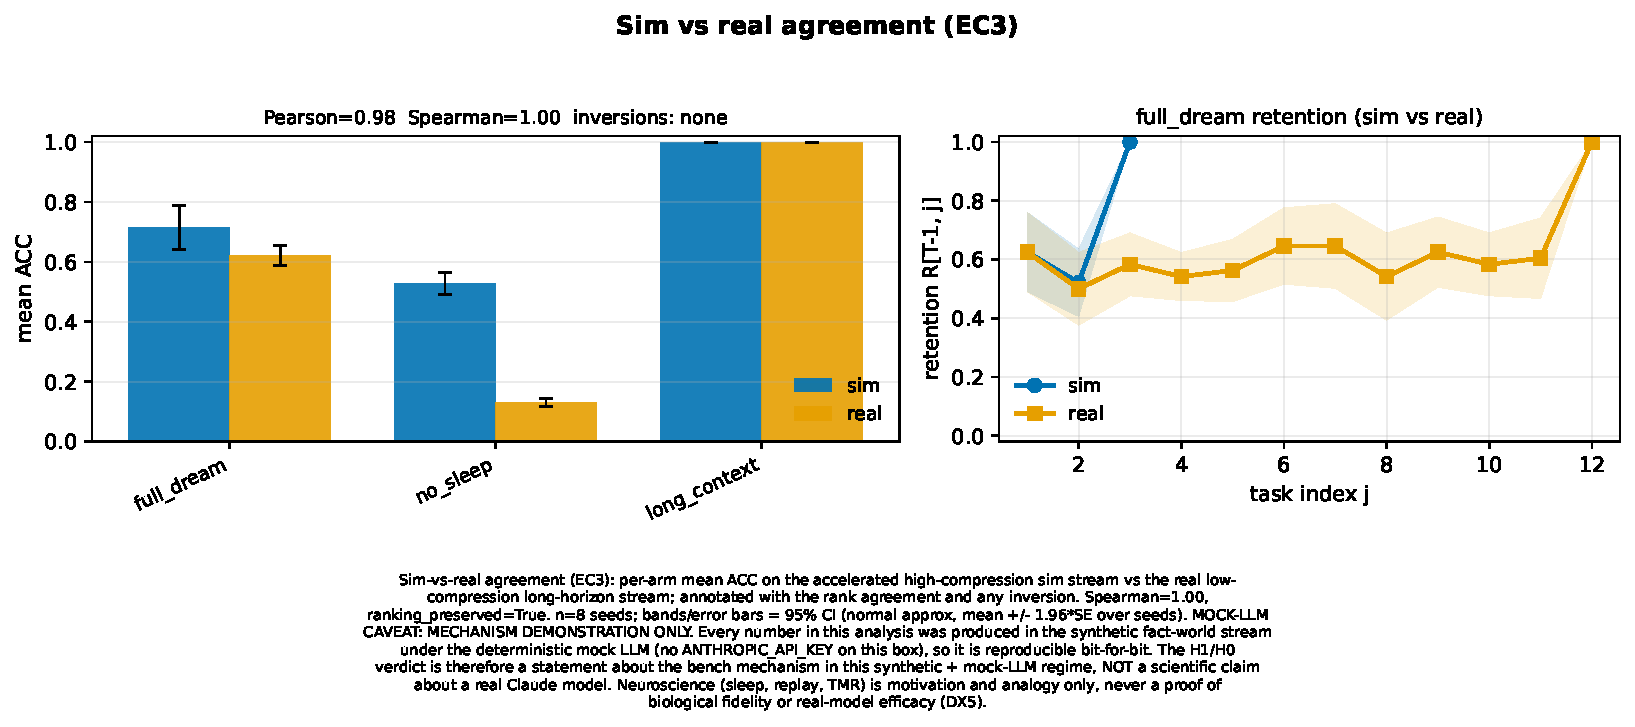
\includegraphics[width=0.82\linewidth]{sim_vs_real.pdf}
  \caption{Sim-vs-real agreement: per-arm mean ACC on the accelerated
  high-compression sim stream vs the real low-compression long-horizon stream,
  annotated with rank agreement and any inversion (Spearman $=\SWsimSpearman$;
  ranking preserved). $n=\SWnSeeds$ seeds; error bars are 95\% CIs (normal
  approximation over seeds). \MockCaveat}
  \label{fig:simreal}
\end{figure}

\paragraph{Interpretation.} In the mock-LLM mechanism-demonstration regime, the
apparatus does what it was built to do: each operator is independently
controllable, consolidation provably moves signal into a durable store, prune
quality is measured against ground truth and is decoupled from accuracy, and the
honest cost picture (long-context dominance on raw accuracy) is surfaced rather
than buried. What these results do \emph{not} establish --- and cannot, under a
mock LLM --- is that a real Claude model would show the same effect, or that the
effect would survive a real summariser's nondeterminism and drift. That is the
experiment the bench is built to run next.

\section{Limitations}\label{sec:limitations}

We state the threats to validity plainly; several bound the claims sharply.

\paragraph{Mock-LLM regime (the dominant caveat).} Every quantitative result in
this paper was produced under a \emph{deterministic mock LLM}, because no live
model key was present on the run machine. This is a deliberate honesty-by-design
choice --- it makes the entire grid byte-reproducible --- but it means the
results are a \textbf{mechanism demonstration in the synthetic, mock-LLM regime}:
they show that the apparatus, its operators, its metrics, and its statistics
behave as designed, and nothing more. They are \emph{not} measurements of a real
Claude model. In particular, the very large primary effect ($d=\SWprimaryD$) and
the near-zero dispersion of the stability control are artifacts of a noiseless
mock summariser; a real model would introduce sampling variance, summarisation
drift, and refusals that the mock cannot. No efficacy claim about a real model
should be read into any number here.

\paragraph{Frozen-weights scope.} We study \emph{memory} consolidation for
\textbf{frozen-weights} agents: the model is never fine-tuned, RLHF'd, or
retrained, and ``consolidation'' refers entirely to operations on an external
memory. Findings therefore say nothing about weight-level continual learning,
and the EWC-spirit protection here is a memory-write flag, not a parameter
penalty.

\paragraph{Sim-time-compression validity.} Most runs use accelerated ``sim-time''
cycles for cheap iteration, validated against a few real low-compression
long-horizon runs. We report the sim-vs-real agreement explicitly
(Section~\ref{sec:results}): the ranking is preserved here (Spearman
$\SWsimSpearman$), but the maximum absolute mean-ACC divergence is
$\SWsimMaxDiv$, which is not negligible. A documented inversion at larger scale
would be a finding, not a bug; we have not swept far enough to exclude one.

\paragraph{Proprietary-model reproducibility.} Real runs would depend on a
proprietary model behind an API. LLM calls are nondeterministic even at
temperature~0, pinned snapshots are eventually deprecated, and exact transcripts
cannot be guaranteed reproducible across snapshots. We mitigate (pinned model
id, multi-seed dispersion, a temperature-0 stability control, archived
transcripts) rather than assume reproducibility, but the caveat is real for any
non-mock run.

\paragraph{Scenario and domain scope.} Results are confined to a single
synthetic, task-incremental stream; each stream is tagged with exactly one
continual-learning scenario and we perform \emph{no} cross-scenario aggregation
\citep{vandeven2022threetypes}. We do not run a secondary ``second-brain'' domain
in this version, and the long-context comparison was swept only over
$L\in\{\SWcrossoverLengths\}$ --- so the absence of a crossover is a statement
about that range, not a universal claim. External validity to natural data,
other scenarios, and longer streams is untested.

\paragraph{No biological-fidelity claim.} Neuroscience supplies the bench's
testable mechanisms and metaphors --- replay, transfer, downscaling, generative
augmentation, TMR --- and nothing more. We do \emph{not} claim that Slow Wave
models the brain, that its operators are biologically faithful, or that any
result transfers to biology. The TMR comparison in particular is to a benchmark
effect size, via a prioritized-replay analogue, not a cued-reactivation protocol.

\section{Reproducibility}\label{sec:repro}

We follow the NeurIPS reproducibility program and its checklist
\citep{pineau2021reproducibility}. Every run emits a JSON manifest recording the
exact model id and sampling parameters, the embedding model, version, and
dimension, all hyperparameters and search ranges, the seed list, the git commit
hash, wall-clock and token/compute cost, and the sim-time compression factor
(the full schema is enumerated in Appendix~\ref{app:repro}). Every figure and
every in-text number in this paper is regenerated from the committed Phase~5
result by a script: the figures by \texttt{slow\_wave.paper.figures} and the
numbers and the per-arm table (Table~\ref{tab:arms}) by
\texttt{slow\_wave.paper.numbers}, which the manuscript \texttt{\textbackslash
input}s rather than hard-coding values. The headline figures regenerate in one
command (\texttt{make repro-figures}), the full grid + analysis + figures in
\texttt{make repro-phase5}, and the entire manuscript --- numbers, figures, and
PDF --- in \texttt{make repro-paper} (\texttt{scripts/build\_paper.sh}). Because
the grid runs under a deterministic mock LLM when no API key is present, all
non-LLM artifacts (embeddings, sampling order, file layout, metrics) are
byte-reproducible across runs with the same config and seeds; any
LLM-dependent field is flagged as such in the manifest. The preregistration,
datasheet, model card, prompts, hyperparameters, and manifest schema are
provided in Appendices~\ref{app:datasheet}--\ref{app:repro}. We note the
standing caveat for any \emph{real}-model run: LLM nondeterminism and snapshot
deprecation mean transcripts are mitigated, not guaranteed reproducible
(Section~\ref{sec:limitations}).

\section{Conclusion}\label{sec:conclusion}

Slow Wave is, to our knowledge, the first mechanism-decomposed continual-learning
bench for LLM-agent memory with controlled distractors and ground-truth
relevance: an apparatus whose four sleep-inspired operators are independently
ablatable, a preregistered, budget-controlled control battery with a
ground-truth-blind negative control and an oracle ceiling, and a metric suite
that measures consolidation \emph{quality} --- prune precision and recall against
known relevance --- decoupled from downstream accuracy. Under a deterministic
mock LLM the apparatus behaves as designed: the full dream cycle improves final
accuracy over the no-sleep baseline on the preregistered primary endpoint
($\Delta=\SWprimaryDiff$), with the registered secondary contrast confirming it
also beats a replay-only control --- at higher token and memory cost, so these are
cost-effectiveness results on the accuracy-vs-compute Pareto frontier, not
matched-budget wins --- and a replay-targeting analogue moves signal into durable
memory as designed (its standardised lift against the sleep-TMR benchmark is
reported but inflated by the mock's determinism). Reported with equal weight, two
cost-unfavourable findings bound the result: an uncapped long-context baseline
dominates on raw accuracy at maximum memory cost with no cost-adjusted crossover in the
swept range, and a simpler deployable shallow-synthesis control
(\texttt{reflection}) attains higher accuracy than the full cycle at lower token
cost --- so the full cycle is the mechanism-decomposable arm, not the cost-optimal
deployable one. We emphasise that these are mechanism
demonstrations in the synthetic, mock-LLM regime, not claims about a real Claude
model, and that neuroscience here is motivation, never proof.

The natural next steps are to run the same preregistered protocol against a real
frozen-weights model (re-checking whether the consolidation effect and its
token/memory cost, the TMR
analogue, and the absence of a long-context crossover survive a real
summariser's nondeterminism and drift), to sweep longer streams in search of a
crossover, to add a second ``second-brain'' domain for external validity, and to
expose the substrate through a production memory tool or MCP for a realism
variant. The apparatus, preregistration, manifests, and one-command reproduction
are released so that others can extend the protocol --- and so that a negative
result, if it comes, is as informative and as reproducible as a positive one.


\bibliographystyle{plainnat}
\bibliography{references}

\appendix
\section{Datasheet for the Synthetic Stream}\label{app:datasheet}

Following \citet{gebru2021datasheets}. The bench emits a fresh datasheet per
stream; the fields below describe the streams used in this paper (the
distractor-heavy primary regime; other regimes differ only in label mix).

\paragraph{Motivation.} The dataset is a \emph{synthetic continual task stream}
created to measure the quality of memory consolidation against known
ground-truth relevance --- the only substrate on which pruning precision/recall
is directly measurable and confounds are controllable. It was created by the
Slow Wave project for this study; no external funding or third party is involved.

\paragraph{Composition.} Each instance is either a \emph{task} or an
\emph{ingest item}. Every item carries exactly one ground-truth relevance label
$\in\{\texttt{signal},\texttt{distractor},\texttt{noise}\}$. \texttt{signal}
items are $(\text{subject},\text{attribute},\text{value})$ facts that answer
probe queries; \texttt{distractor} items are plausible but mission-irrelevant
facts drawn from a separate namespace; \texttt{noise} items are random tokens
with no fact. A stream has $n\_\text{tasks}=5$ tasks of
$\text{items\_per\_task}=40$ items (200 items) in the primary configuration,
with $8$ subjects/task, $4$ attributes, $12$ values, a distractor namespace of
$64$, and a noise vocabulary of $128$. The label mix for the primary
(distractor-heavy) regime is signal $0.34$ / distractor $0.40$ / noise $0.26$.
A held-out probe set ($6$ probes/task) is decoupled from the online stream. The
dataset is self-contained and synthetic; it contains no personal, sensitive, or
confidential data (Non-Goal NG5).

\paragraph{Collection / generation process.} Items are generated procedurally
and are \emph{byte-deterministic given a stream seed}: the same seed yields a
byte-identical stream and datasheet. Temporal structure (recency bias, drift)
and contradiction rate are configurable (all $0$ in the primary configuration).
Each stream is tagged with exactly one continual-learning scenario
(here \texttt{task-incremental}; \citealp{vandeven2022threetypes}); no
cross-scenario mixing is permitted.

\paragraph{Labeling and the confound guard.} Ground-truth relevance labels are
assigned at generation time and stored in an \emph{offline-only} label sidecar.
A confound guard (functional requirement FR1.6) enforces --- in code, asserted
by test, and checked by an import firewall --- that these labels are unreachable
from any online retrieval or priority code path, preventing an oracle-replay
leak. Only offline scoring may read them.

\paragraph{Uses.} The stream supports continual-learning evaluation (the
accuracy matrix $R[i,j]$), mechanism-level prune-quality scoring (precision /
recall / F1 of discarding distractors vs.\ retaining signal), and cost/footprint
measurement. It is \emph{not} intended as a natural-language benchmark and makes
no claim of external validity to natural data.

\paragraph{Distribution and maintenance.} The generator, configs, and the
committed run manifests ship with the repository; any stream is regenerable from
its seed and config. The datasheet emitter is versioned with the codebase; the
authoritative interface is documented in the repository's Phase~1 contract.

\section{Model Card}\label{app:modelcard}

Following \citet{mitchell2019modelcards}. This card covers the two models the
bench uses: the (frozen) reasoning/summarisation LLM and the local embedding
model.

\paragraph{Model details.} The configured reasoning and dream-summarisation
model is \texttt{\SWmodelID} (a pinned Claude snapshot), called with sampling
temperature $0.0$, \texttt{max\_tokens}~$=64$, \texttt{top\_p} unset, and
\texttt{effort} unset. \textbf{The runs in this paper used a deterministic mock
LLM} (\texttt{mocked}=\SWmodelMocked), because no \texttt{ANTHROPIC\_API\_KEY}
was present on the run machine: the mock returns text fully determined by
$(\text{model id},\text{system},\text{prompt})$, so the pipeline is
byte-reproducible. Consequently every number is a \emph{mechanism demonstration},
not a measurement of the real snapshot (Section~\ref{sec:limitations}). The
local embedding model is a hash bag-of-words backend (\texttt{hash-bow-v1},
dimension $384$, version $1.0$); it is deterministic given its input and
CPU-friendly. (A \texttt{sentence-transformers} backend such as
\texttt{bge-small-en-v1.5} is supported as a configuration option but was not
used for these committed runs.)

\paragraph{Intended use.} The models are a measurement vehicle for studying
external-memory consolidation around a \emph{frozen-weights} agent. Intended use
is research on the bench's synthetic stream. Out-of-scope: production deployment,
any use requiring biological fidelity, and any efficacy claim beyond the tested
synthetic, mock-LLM regime.

\paragraph{Factors and metrics.} Relevant factors are the distractor regime,
the stream/sampling seed, and the dream-operator configuration. Metrics are the
continual-learning set (ACC, BWT, FWT, per-task forgetting;
\citealp{lopezpaz2017gem,chaudhry2018riemannian}), the mechanism-level prune
precision/recall/F1 and decay-vs-relevance calibration, cost (tokens, memory
vectors/bytes, p95 latency, wall-clock, sim-time compression), generator
fidelity/drift, and the TMR-style retention lift.

\paragraph{Training data.} \textbf{None: weights are frozen.} No fine-tuning,
RLHF, or retraining is performed; ``consolidation'' acts only on the external
memory. The local embedder is not trained by this project.

\paragraph{Ethical considerations and caveats.} The synthetic stream contains no
personal or sensitive content (NG5). The dominant caveat is the mock-LLM regime
(above). For any real-model run, the standing caveats are LLM nondeterminism even
at temperature~0, eventual snapshot deprecation, and summarisation drift; the
bench mitigates these with a pinned model id, multi-seed dispersion, a
temperature-0 stability control, a memory-drift detector, and archived
transcripts, rather than assuming reproducibility.

\section{Hyperparameters, Search Ranges, and Prompts}\label{app:hyper}

All values are taken from the committed experiment config
(\texttt{configs/phase5\_full.yaml}) and the run manifests.

\paragraph{Stream and memory.} Scenario \texttt{task-incremental}; $5$ tasks
$\times$ $40$ items; $8$ subjects/task, $4$ attributes, $12$ values, $6$
probes/task; distractor namespace $64$, noise vocabulary $128$, $8$ noise
tokens; contradiction rate $0$, drift $0$, recency bias $0$. Episodic capacity
$60$ (bounded, so the no-sleep baseline forgets); archival tier enabled;
retrieval policy recency\,$\times$\,importance\,$\times$\,relevance with
top-$k=16$ and recency half-life $64$.

\paragraph{Dream engine.} All four operators enabled in \texttt{full\_dream}:
replay (strategy \emph{prioritized}, sample size $24$), transfer (batch size
$8$, CLS interleaving on at ratio $0.5$), downscale (decay function
\emph{exponential}, re-potentiation boost $1.5$), generative-augment
($4$ pseudo-episodes/cycle, kinds cycling through paraphrase / abstraction /
counterfactual). Conflict/unlearning off; sleep every $1$ task; sleep-pressure
mode \emph{fixed}.

\paragraph{Evaluation.} Nine arms (Section~\ref{sec:protocol}); seeds
$\{0,\dots,7\}$ ($n=\SWnSeeds$); matched-budget controller enabled with tolerance
$0.15$ (the realised grid is out of tolerance for \texttt{full\_dream}, so
\texttt{budget\_matched} is false and the accuracy-vs-compute Pareto frontier is
the operative artifact; Section~\ref{sec:results});
$10{,}000$ bootstrap resamples at the $0.95$ CI level; stats seed $0$; stability
repeats $3$; drift rounds $3$; A/A reference arm \texttt{no\_sleep}; treatment
\texttt{full\_dream}; baseline \texttt{no\_sleep}; primary endpoint
\texttt{\SWprimaryEndpoint}.

\paragraph{Search ranges / swept grids.} The study sweeps three explicit grids
(the manifest \texttt{search\_ranges} block is empty because the sweep is
expressed as the grids below, each enumerated and logged with no silent caps):
\begin{itemize}
  \item \textbf{Distractor regimes} (signal / distractor / noise): signal-rich
  $0.70/0.20/0.10$, balanced $0.50/0.30/0.20$, distractor-heavy
  $0.34/0.40/0.26$ (the preregistered primary regime).
  \item \textbf{Stream-length sweep} (long-context crossover):
  $L\in\{\SWcrossoverLengths\}$ over key arms
  \{\texttt{full\_dream}, \texttt{long\_context}, \texttt{no\_sleep}\}.
  \item \textbf{Sim-vs-real}: accelerated sim ($\SWsimNtasksSim$ tasks,
  compression $\approx\SWsimCompression\times$) vs.\ real long-horizon
  ($\SWsimNtasksReal$ tasks, compression $1\times$) over key arms
  \{\texttt{full\_dream}, \texttt{no\_sleep}, \texttt{long\_context}\}.
\end{itemize}

\paragraph{Prompts.} The dream \emph{transfer} (NREM distillation) prompt is
built deterministically per batch:
\begin{quote}\small\ttfamily
You are consolidating recent episodic observations into durable, generalizable
semantic memory during a sleep cycle.\\[2pt]
New observations to consolidate:\\
\ \ 1. <observation>\ \ldots\\[2pt]
Prior consolidated knowledge (context only --- do not rewrite):\\
\ \ 1. <prior entry>\ \ldots\ \ (only when CLS interleaving is on)\\[2pt]
Write one concise paragraph that distills the new observations, integrating them
with the prior knowledge without contradicting it.
\end{quote}
The \emph{generative-augment} (REM) prompt for each selected source is
\texttt{"<kind> of: <source content>"}, where \texttt{<kind>} cycles through
\texttt{paraphrase}, \texttt{abstraction}, \texttt{counterfactual}. The per-task
agent \emph{reasoning} prompt is \texttt{"Review the recent observations and note
any facts worth remembering."} (optionally suffixed with retrieved memory
context); this call is for telemetry/realism only --- probe answers are read
deterministically from memory by exact-key lookup, never from the LLM, which is
what keeps the mock-LLM pipeline byte-reproducible. A direct consequence is that
any arm retaining a probed key answers it correctly regardless of model behaviour:
\texttt{long\_context} (unbounded episodic capacity) keeps every key and so attains
the maximum possible final accuracy by construction (Table~\ref{tab:arms}), and the
consolidation arms affect accuracy solely through what they retain --- so the
continual-learning scores here measure a retention policy, not probe-time reasoning
(Section~\ref{sec:limitations}).

\section{Reproducibility Appendix}\label{app:repro}

This appendix gives the information requested by the NeurIPS reproducibility
checklist \citep{pineau2021reproducibility}: the pinned model, the full
hyperparameters and swept grids, the prompts, the per-run manifest schema, and
the one-command reproduction.

\paragraph{Pinned model and environment.} Reasoning/summarisation model
\texttt{\SWmodelID} (pinned snapshot), sampling temperature $0.0$,
\texttt{max\_tokens}~$=64$; runs executed under the deterministic mock LLM
(\texttt{mocked}=\SWmodelMocked). Local embedder \texttt{hash-bow-v1}, dimension
$384$. Python $3.12$; package version $0.1.0$; statistics implemented in pure
NumPy. Committed result at git \texttt{\SWgitCommit}.

\paragraph{Hyperparameters, search ranges, and prompts.} Given in full in
Appendix~\ref{app:hyper} (stream, memory, dream-engine, and evaluation
hyperparameters; the three swept grids; and the transfer / augment / reasoning
prompts).

\paragraph{Per-run manifest schema (FR6.1).} Every run writes a JSON manifest
whose top-level keys are: \texttt{manifest\_version}, \texttt{experiment},
\texttt{run\_id}, \texttt{config\_hash}, \texttt{created\_at};
\texttt{model} (\texttt{id}, \texttt{mocked}, and \texttt{sampling}:
\texttt{temperature}/\texttt{max\_tokens}/\texttt{top\_p}/\texttt{effort});
\texttt{llm} (\texttt{model\_id}, \texttt{mocked}, token counts, output
\texttt{text\_sha256});
\texttt{embedding} (\texttt{backend}, \texttt{model}, \texttt{version},
\texttt{dim});
\texttt{seeds} (master + per-arm derivation) and \texttt{seed\_list};
\texttt{hyperparameters} and \texttt{search\_ranges};
\texttt{cost} (\texttt{api\_calls}, \texttt{tokens}.\{input,output,total\},
\texttt{wall\_clock\_s}, and per-arm memory vectors/bytes, retrieval calls, and
p95 latency in the results block);
\texttt{git} (\texttt{commit}, \texttt{branch}, \texttt{dirty});
\texttt{sim\_time} (\texttt{compression\_factor});
\texttt{platform}, \texttt{python\_version}, \texttt{package\_version};
\texttt{results} (the full per-(arm,seed) experiment: $R[i,j]$, continual
metrics, prune quality, calibration, footprint, statistics, A/A, prereg primary
endpoint, drift, stability); and
\texttt{nondeterministic\_fields}, which explicitly lists the fields that may
vary under a real LLM --- \texttt{created\_at}, \texttt{cost.wall\_clock\_s},
output token counts, \texttt{llm.text\_sha256}/\texttt{text\_preview}, the git
fields, and per-step latencies --- so a reader knows exactly which values are not
byte-stable. (Under the mock LLM even most of these are stable run-to-run; the
field merely marks what is \emph{permitted} to vary.)

\paragraph{One-command reproduction.} From a clean checkout with the package
installed (\texttt{pip install -e ".[viz]"}):
\begin{itemize}
  \item \textbf{Headline figures} (the EC2 one-command regeneration from the
  committed result): \texttt{make repro-figures}, i.e.\
  \texttt{python -m slow\_wave.paper.figures --result phase5/phase5\_result.json
  --out paper/figures}.
  \item \textbf{In-text numbers and the per-arm table}:
  \texttt{make repro-numbers}, i.e.\
  \texttt{python -m slow\_wave.paper.numbers --result phase5/phase5\_result.json
  --out paper/generated} (the manuscript \texttt{\textbackslash input}s these, so
  no number is hand-transcribed).
  \item \textbf{Full grid + analysis + figures}: \texttt{make repro-phase5}.
  \item \textbf{The entire manuscript} (numbers + figures + PDF):
  \texttt{make repro-paper} (\texttt{scripts/build\_paper.sh}).
\end{itemize}
Because the grid runs under the deterministic mock LLM when no API key is
present, every non-LLM artifact is byte-reproducible across runs with the same
config and seeds; the \texttt{nondeterministic\_fields} list flags everything
that is not. This is a mechanism-demonstration reproduction
(Section~\ref{sec:limitations}); a real-model run is reproducible only up to LLM
nondeterminism, which is why the bench reports dispersion, a temperature-0
stability control, and a memory-drift detector rather than assuming
bit-for-bit determinism.


\end{document}
